\documentclass{beamer}
\usetheme[compress]{Padova}
\usepackage{presentazione}
\usepackage{tikz}
\usetikzlibrary{arrows}
\addbibresource{msbd.bib}
\title{\textsc{Classificazione di attività motorie tramite accelerometro del cellulare}}
\author{Luisa Galtarossa\and Alberto Grassi\and Anna Montin\and Daniele Zago}
\date{}

\newcommand{\getsection}{\color{white}\insertsection}

\begin{document}
\begin{frame}
\titlepage
\end{frame}

\section{Introduzione}
\begin{frame}{Il problema analizzato}
Ormai con il cellulare è possibile fare moltissime cose. 
Cancellare messaggi, avere più giga\dots È tutto possibile con un solo shake.\\
\smallskip
Ma come si può riconoscere uno shake?
\begin{figure}[H]

\includegraphics[width=0.4\textwidth]{./images/vodafoneshake.png}
\end{figure}
\end{frame}

\begin{frame}{La nostra idea}
Riconoscere uno shake tra diverse attività motorie.\\
\smallskip
\begin{columns}[T] % align columns
\begin{column}{.48\textwidth}
Le attività analizzate sono:
\begin{itemize}
\item Camminata
\item Camminata con cellulare in tasca
\item Corsa
\item Corsa con cellulare in tasca
\item Utilizzo a riposo
\item Salti
\item Salita e discesa di scale
\end{itemize}
\end{column}%
\hfill%
\begin{column}{.4\textwidth}
\begin{figure}[H]
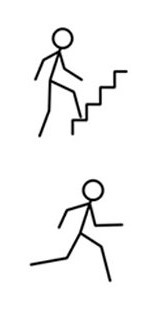
\includegraphics[width=0.6\textwidth]{./images/attivit.jpg}
\end{figure}
\end{column}%
\end{columns}
\end{frame}

\begin{frame}{Raccolta dati}
I dati sono stati raccolti tramite l'applicazione \texttt{PhonePi} \cite{kumarPhonePiSampleServer2019}.\\
\smallskip
Questa fornisce l'accelerazione in forma vettoriale ad ogni istante $t$.
\[
\vec{a}_t = \begin{pmatrix}
a_{xt} \\ a_{yt} \\ a_{zt}
\end{pmatrix}
\]
\end{frame}

\begin{frame}{Accelerazione}
L'accelerazione viene calcolata come $\|\vec{a_t}\| =\sqrt{a_{xt}^2+a_{yt}^2+a_{zt}^2}$.
\begin{figure}[H]
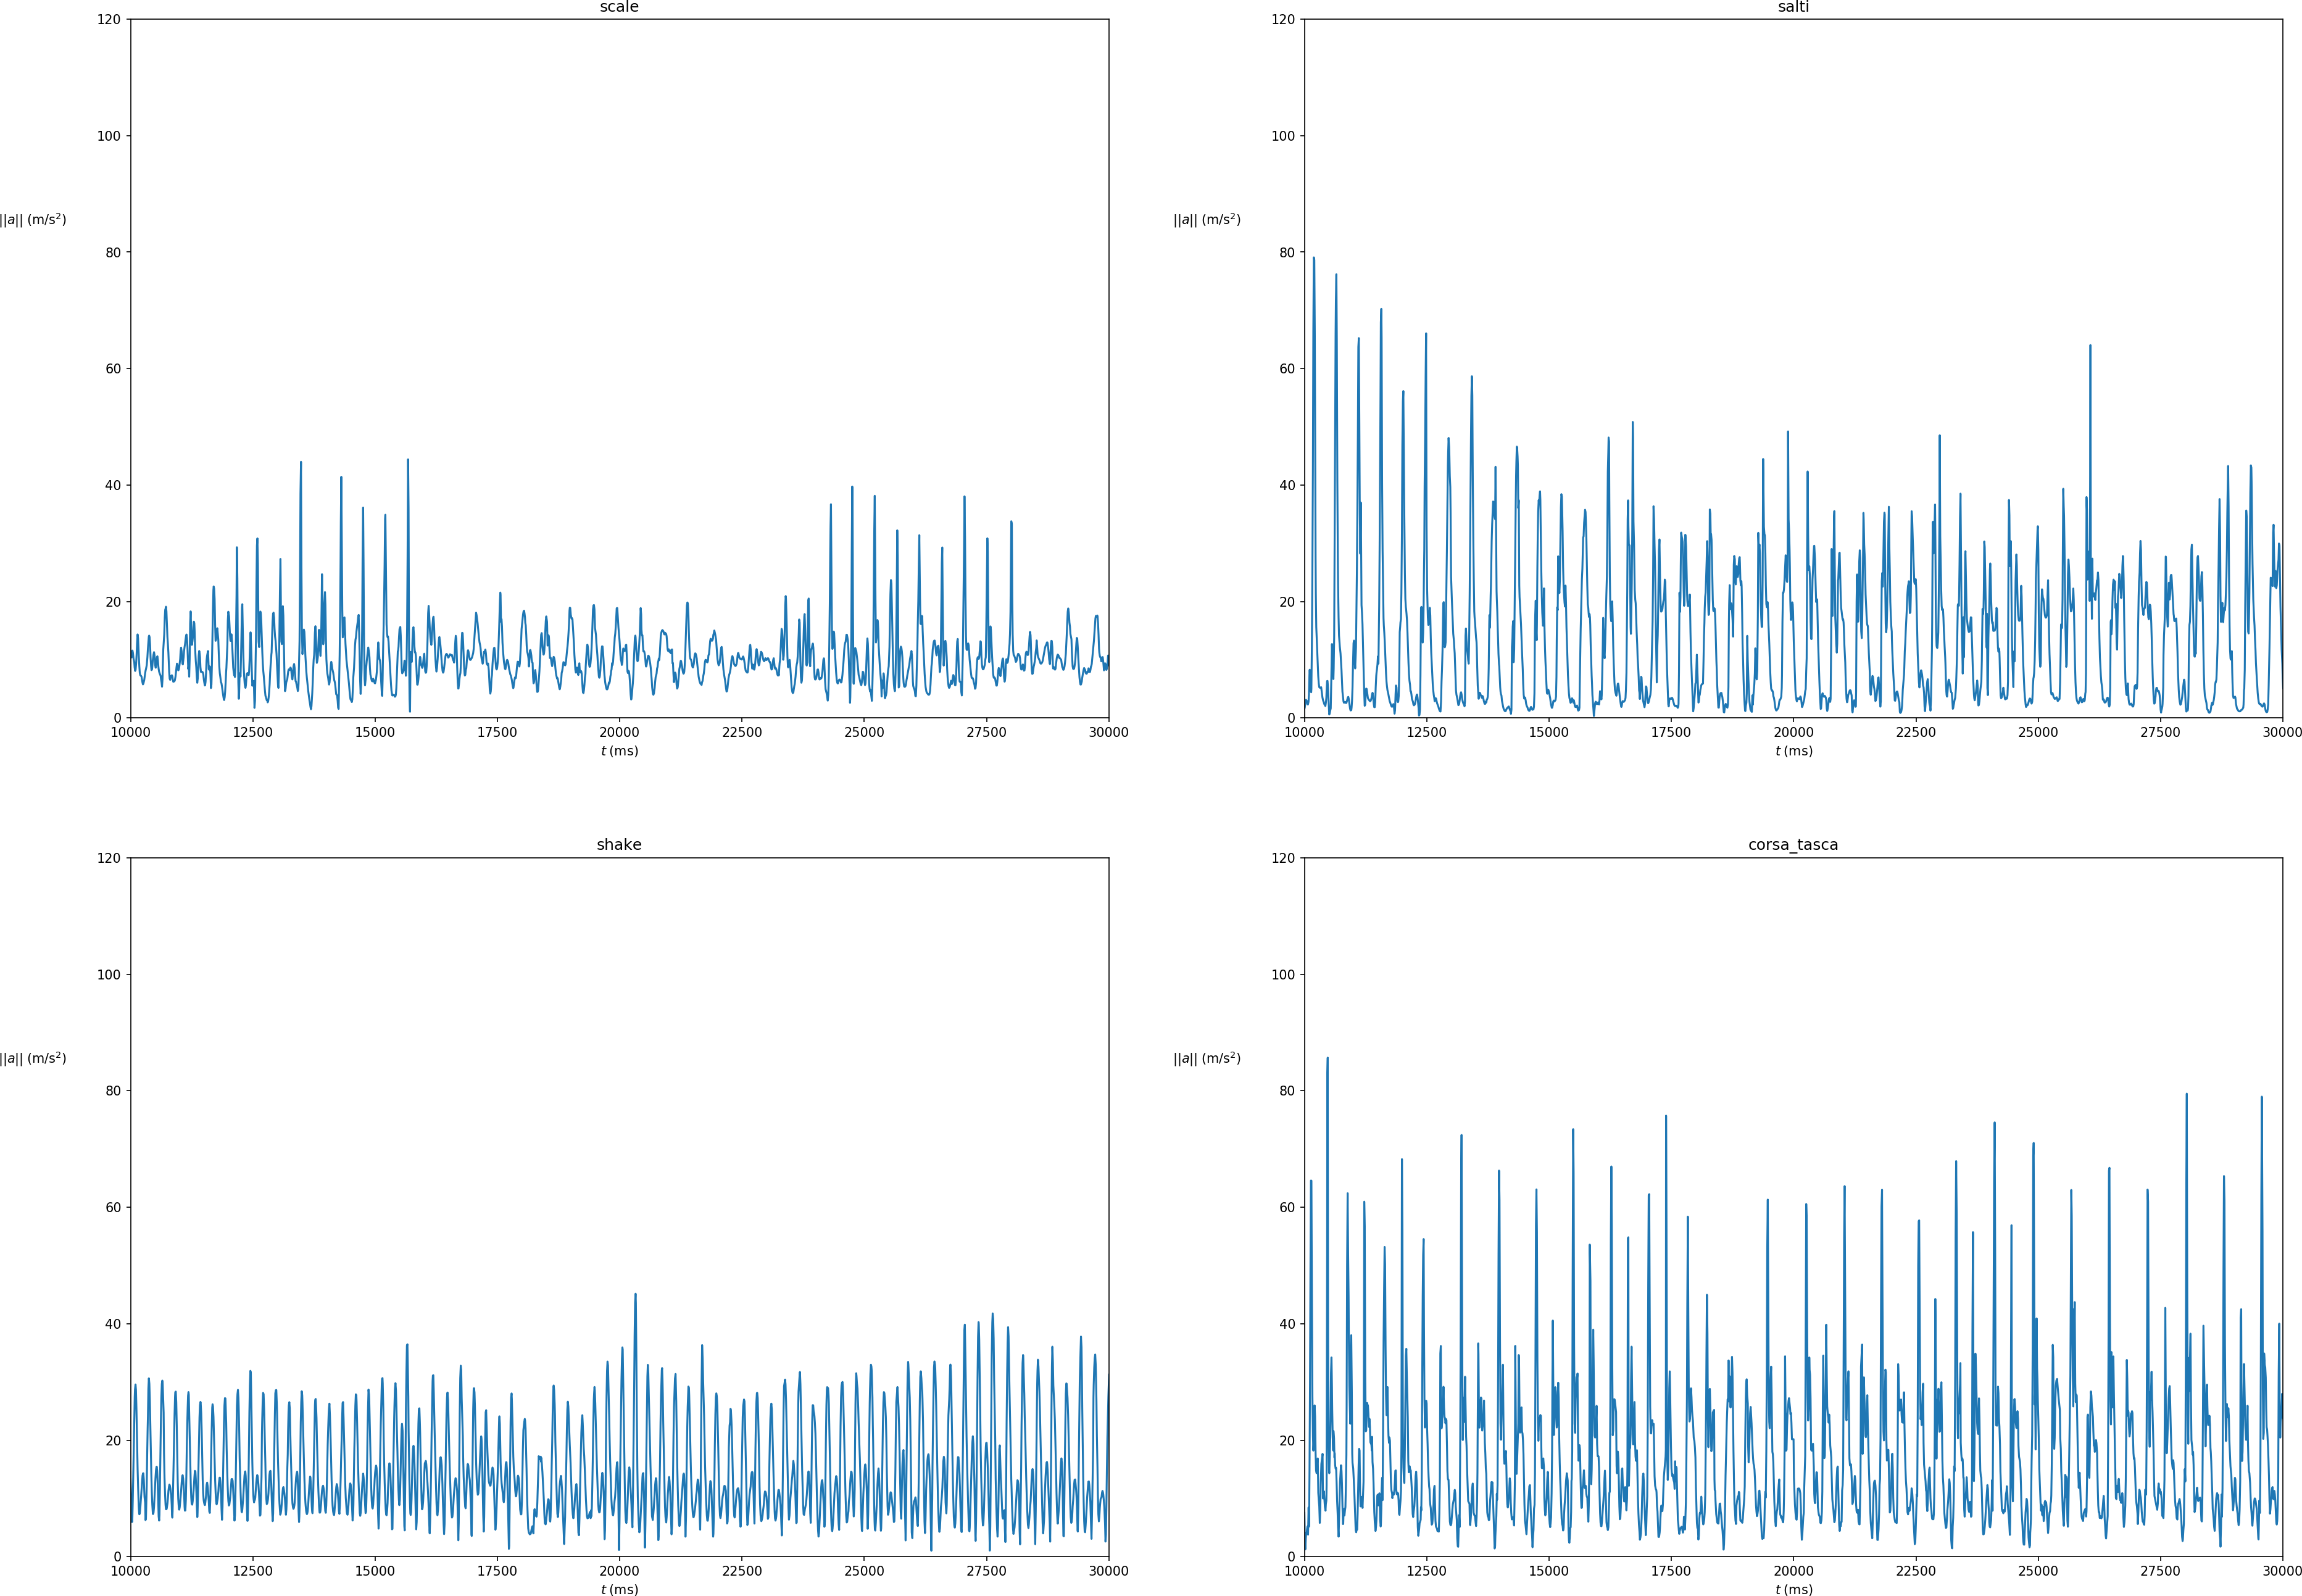
\includegraphics[width=\textwidth]{../figure/espl.png}
\end{figure}
\end{frame}

\section{Esplorativa}
\begin{frame}{Accelerazione}
I dati sono stati suddivisi in intervalli di ampiezza $\SI{1.5}{s}$
\begin{table}[H]
\begin{tabular}{cccccccc}
\toprule
y & $\|\vec{a}_0\|$ & $\|\vec{a}_1\|$ & $\|\vec{a}_2\|$  & $\dots$ & $\|\vec{a}_{149}\|$\\
\midrule
camminata & 5.449 & 5.300 & 5.344 &  $\cdots$ & 13.147\\
camminata & 13.977 & 14.910 & 15.567 &  $\cdots$ & 5.480\\
camminata & 5.608 & 5.868 & 6.143 &  $\cdots$ & 18.227\\
camminata & 19.026 & 18.886 & 18.098 &  $\cdots$ & 6.299\\
$\vdots$ & $\vdots$ & $\vdots$ & $\vdots$ &  $\vdots$ & $\vdots$\\
shake & 11.480 & 14.663 & 16.968 &  $\cdots$ & 8.474\\
\bottomrule
\end{tabular}
\end{table}
\pause Perché non lavorare direttamente con le esplicative $\|\vec{a}_0\|,\dots,\|\vec{a}_{149}\|$?
\end{frame}

\begin{frame}{Accelerazione}
	\begin{figure}[H]
		\centering
		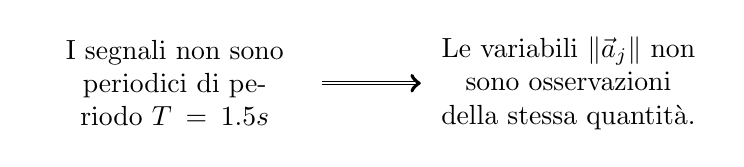
\begin{tikzpicture}
		\node[text width=3.5cm, align=center, rectangle] (a) at (-2.5,0){I segnali non sono periodici di periodo $T = \SI{1.5}{s}$};
		\node[text width=3.5cm, align=center, rectangle] (b) at (2.5,0){Le variabili $\|\vec{a}_j\|$ non sono osservazioni della stessa quantità.};
		\draw[->, double] (a) -- (b);
		\end{tikzpicture}
	\end{figure}
\pause
\textbf{Soluzione}: variabili riassuntive dell'intervallo:
\begin{table}[H]
	\centering
	\begin{tabular}{ll}
		\texttt{minA}& Minimo dell'accelerazione.\\
		\texttt{medA}& Mediana dell'accelerazione.\\
		\texttt{varA}& Varianza dell'accelerazione.\\
		\texttt{maxA}& Massimo dell'accelerazione.\\
		\texttt{meanA}& Media dell'accelerazione.\\
		\texttt{MVDeriv}& Media del valore assoluto della derivata seconda.
	\end{tabular}
\end{table}
\end{frame}

\section{Bibliografia}
\begin{frame}{Bibliografia}
\printbibliography
\end{frame}
\end{document}
